\documentclass[11pt,a4paper]{report}
\usepackage[textwidth=37em,vmargin=30mm]{geometry}
\usepackage{calc,xunicode,amsmath,amssymb,paralist,enumitem,tabu,booktabs,datetime2,xeCJK,xeCJKfntef,listings}
\usepackage{tocloft,fancyhdr,tcolorbox,xcolor,graphicx,eso-pic,xltxtra,xelatexemoji}

\newcommand{\envyear}[0]{2025}
\newcommand{\envdatestr}[0]{2025-01-15}
\newcommand{\envfinaldir}[0]{webdb/2025/20250115/final}

\usepackage[hidelinks]{hyperref}
\hypersetup{
    colorlinks=false,
    pdfpagemode=FullScreen,
    pdftitle={Web Digest - \envdatestr}
}

\setlength{\cftbeforechapskip}{10pt}
\renewcommand{\cftchapfont}{\rmfamily\bfseries\large\raggedright}
\setlength{\cftbeforesecskip}{2pt}
\renewcommand{\cftsecfont}{\sffamily\small\raggedright}

\setdefaultleftmargin{2em}{2em}{1em}{1em}{1em}{1em}

\usepackage{xeCJK,xeCJKfntef}
\xeCJKsetup{PunctStyle=plain,RubberPunctSkip=false,CJKglue=\strut\hskip 0pt plus 0.1em minus 0.05em,CJKecglue=\strut\hskip 0.22em plus 0.2em}
\XeTeXlinebreaklocale "zh"
\XeTeXlinebreakskip = 0pt


\setmainfont{Brygada 1918}
\setromanfont{Brygada 1918}
\setsansfont{IBM Plex Sans}
\setmonofont{JetBrains Mono NL}
\setCJKmainfont{Noto Serif CJK SC}
\setCJKromanfont{Noto Serif CJK SC}
\setCJKsansfont{Noto Sans CJK SC}
\setCJKmonofont{Noto Sans CJK SC}

\setlength{\parindent}{0pt}
\setlength{\parskip}{8pt}
\linespread{1.15}

\lstset{
	basicstyle=\ttfamily\footnotesize,
	numbersep=5pt,
	backgroundcolor=\color{black!5},
	showspaces=false,
	showstringspaces=false,
	showtabs=false,
	tabsize=2,
	captionpos=b,
	breaklines=true,
	breakatwhitespace=true,
	breakautoindent=true,
	linewidth=\textwidth
}






\newcommand{\coverpic}[2]{
    % argv: itemurl, authorname
    Cover photo by #2~~(\href{#1}{#1})
}
\newcommand{\makeheader}[0]{
    \begin{titlepage}
        % \newgeometry{hmargin=15mm,tmargin=21mm,bmargin=12mm}
        \begin{center}
            
            \rmfamily\scshape
            \fontspec{BaskervilleF}
            \fontspec{Old Standard}
            \fontsize{59pt}{70pt}\selectfont
            WEB\hfill DIGEST
            
            \vfill
            % \vskip 30pt
            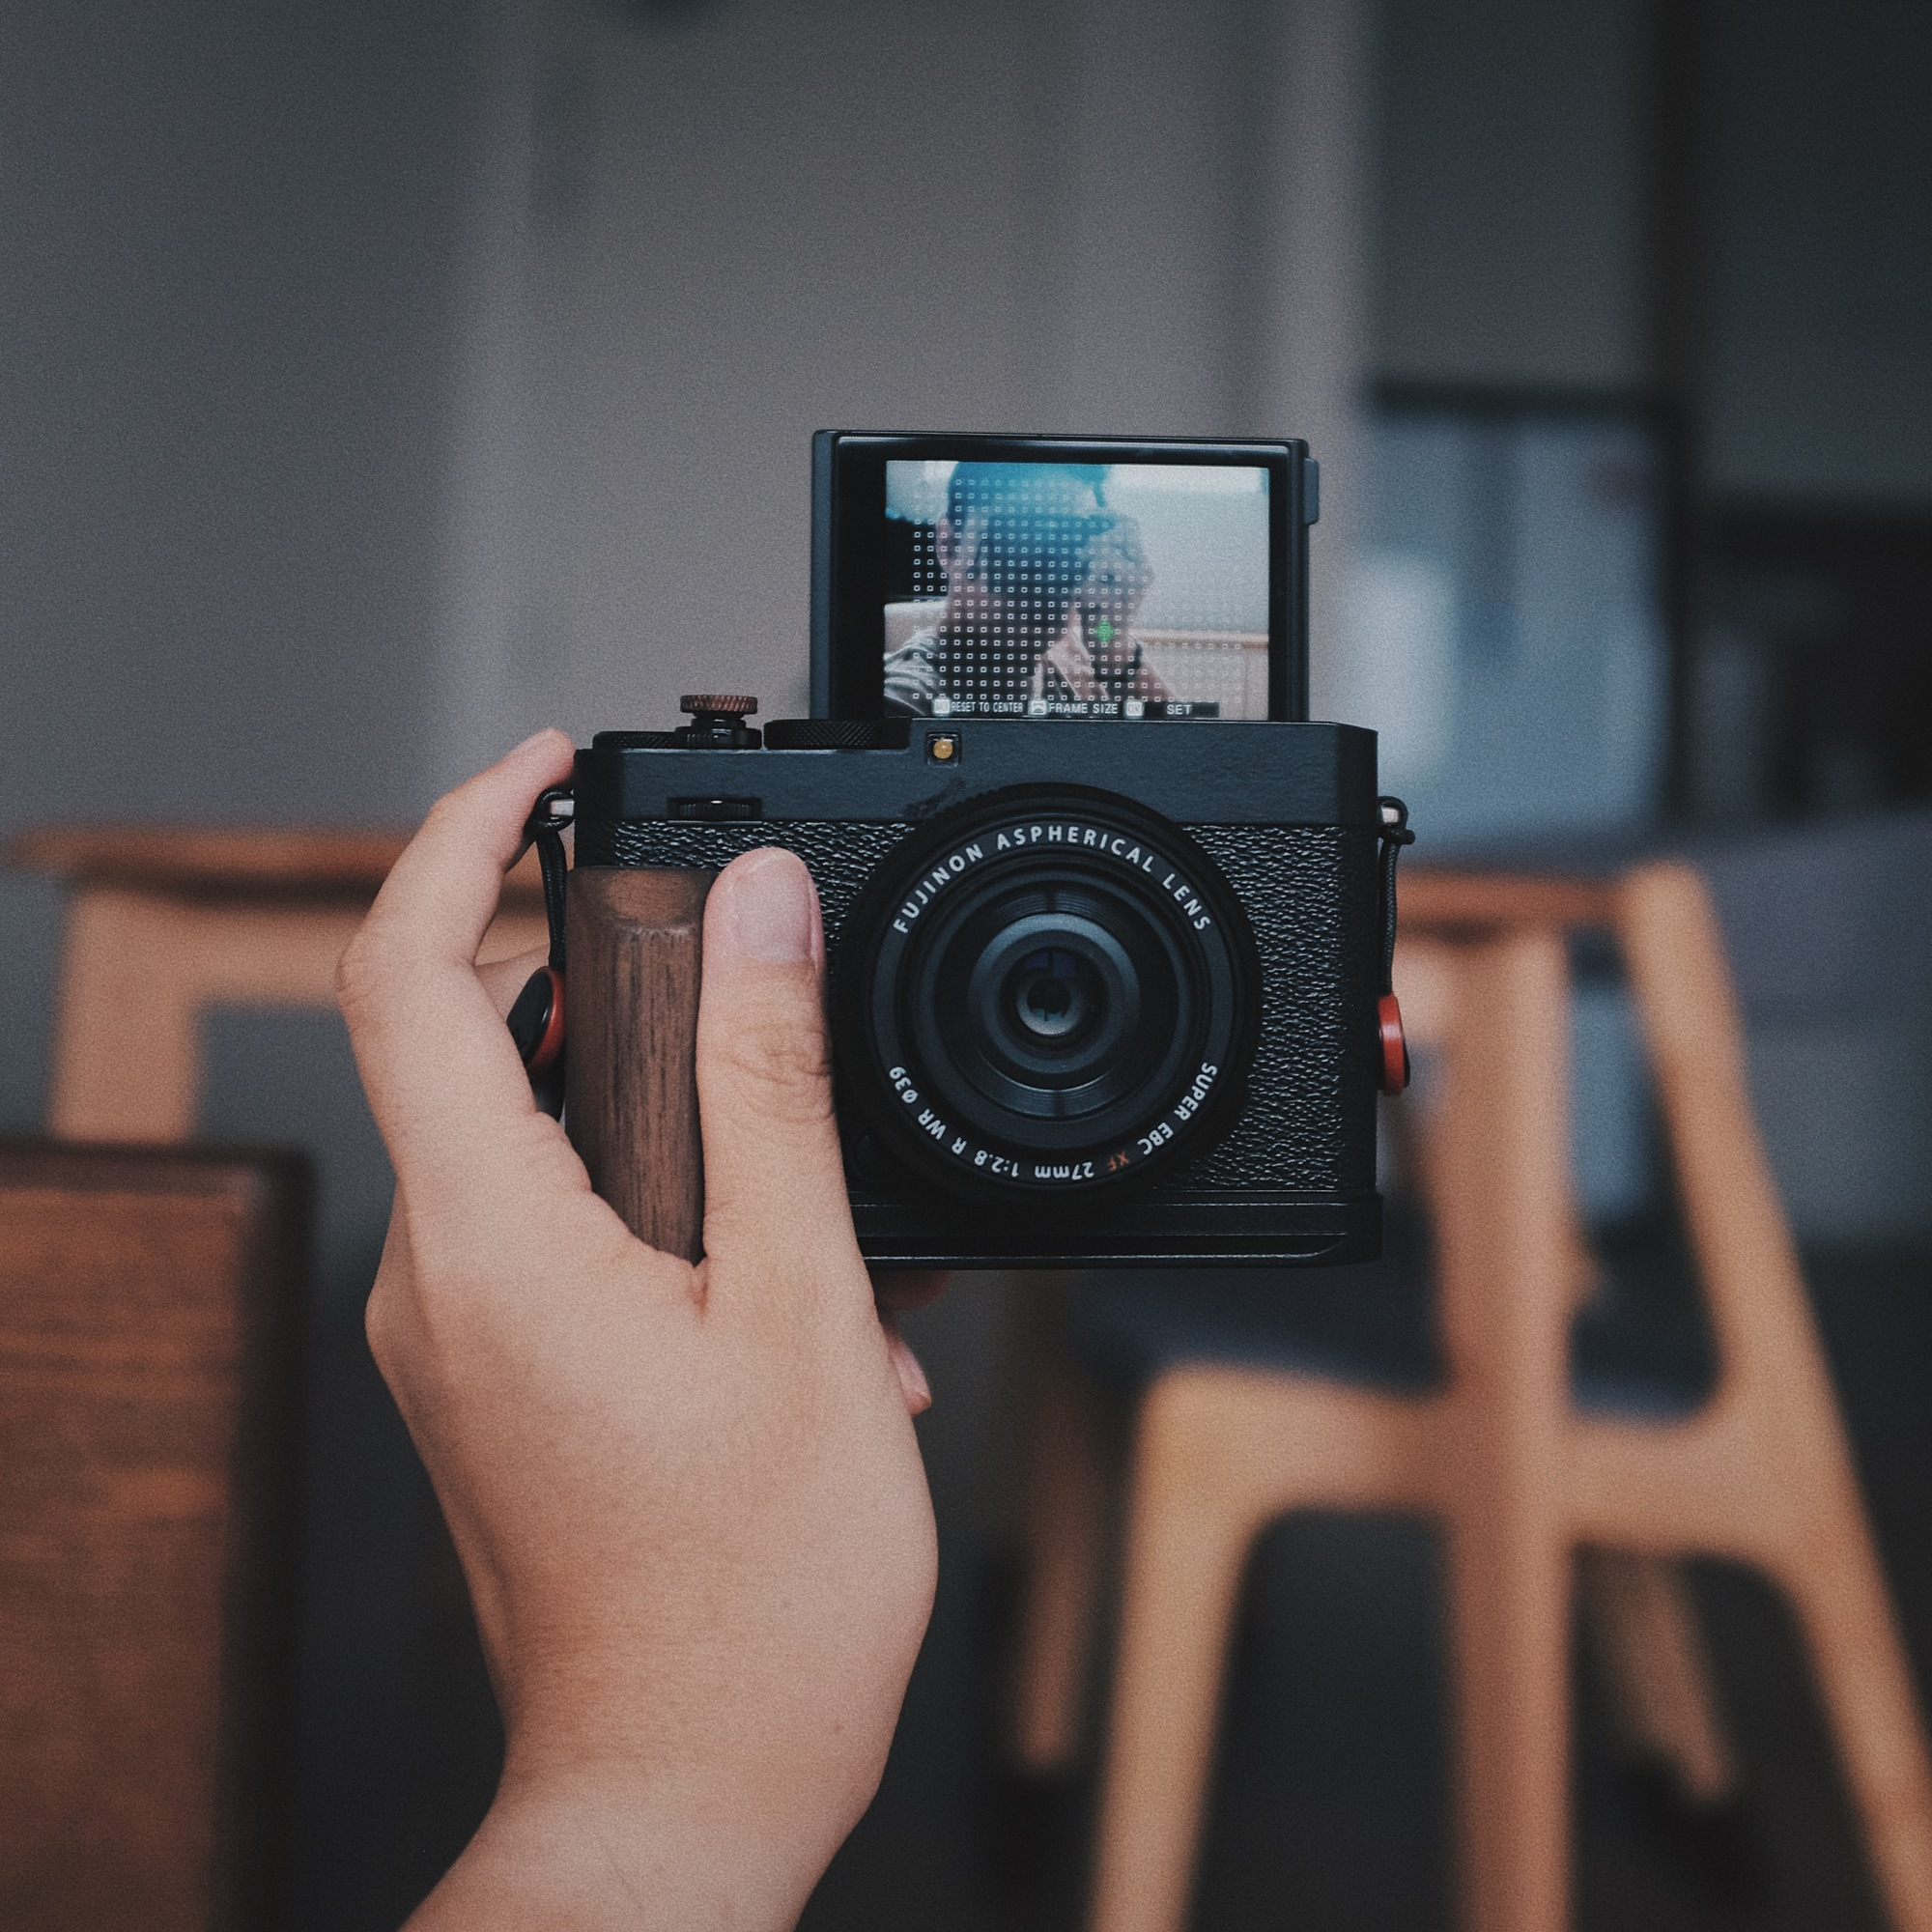
\includegraphics[width=\linewidth]{\envfinaldir/coverpic-prod.jpg}\par
            % \vskip 30pt
            \vfill

            \normalsize\rmfamily\scshape
            \copyright{} The Web Digest Project \hfill\large \envdatestr
        \end{center}
    \end{titlepage}
    % \restoregeometry
}
\newcommand{\simplehref}[1]{%
    \textcolor{blue!80!green}{\href{#1}{#1}}%
}
\renewcommand{\contentsname}{\center\Huge\sffamily\bfseries Contents\par\vskip 20pt}
\newcounter{ipartcounter}
\setcounter{ipartcounter}{0}
\newcommand{\ipart}[1]{
    % \vskip 20pt
    \clearpage
    \stepcounter{ipartcounter}
    \phantomsection
    \addcontentsline{toc}{chapter}{#1}
    % \begin{center}
    %     \Huge
    %     \sffamily\bfseries
    %     #1
    % \end{center}
    % \vskip 20pt plus 7pt
}
\newcounter{ichaptercounter}
\setcounter{ichaptercounter}{0}
\newcommand{\ichapter}[1]{
    % \vskip 20pt
    \clearpage
    \stepcounter{ichaptercounter}
    \phantomsection
    \addcontentsline{toc}{section}{\numberline{\arabic{ichaptercounter}}#1}
    \begin{center}
        \Huge
        \sffamily\bfseries
        #1
    \end{center}
    \vskip 20pt plus 7pt
}
\newcommand{\entrytitlefont}[1]{\subsection*{\raggedright\Large\sffamily\bfseries#1}}
\newcommand{\entryitemGeneric}[2]{
    % argv: title, url
    \parbox{\linewidth}{
        \entrytitlefont{#1}\par\vskip 5pt
        \footnotesize\ttfamily\mdseries
        \simplehref{#2}
    }\vskip 11pt plus 11pt minus 1pt
}
\newcommand{\entryitemGithub}[3]{
    % argv: title, url, desc
    \parbox{\linewidth}{
        \entrytitlefont{#1}\par\vskip 5pt
        \footnotesize\ttfamily\mdseries
        \simplehref{#2}\par\vskip 5pt
        \small\rmfamily\mdseries#3
    }\vskip 11pt plus 11pt minus 1pt
}
\newcommand{\entryitemAp}[3]{
    % argv: title, url, desc
    \parbox{\linewidth}{
        \entrytitlefont{#1}\par\vskip 5pt
        \footnotesize\ttfamily\mdseries
        \simplehref{#2}\par\vskip 5pt
        \small\rmfamily\mdseries#3
    }\vskip 11pt plus 11pt minus 1pt
}
\newcommand{\entryitemHackernews}[3]{
    % argv: title, hnurl, rawurl
    % \parbox{\linewidth}{
    %     \entrytitlefont{#1}\par\vskip 5pt
    %     \footnotesize\ttfamily\mdseries
    %     \simplehref{#3}\par
    %     \textcolor{black!50}{\href{#2}{#2}}
    % }\vskip 11pt plus 11pt minus 1pt
    \begin{minipage}{\linewidth}
            \entrytitlefont{#1}\par\vskip 5pt
            \footnotesize\ttfamily\mdseries
            \simplehref{#3}\par
            \textcolor{black!50}{\href{#2}{#2}}
    \end{minipage}\par\vskip 11pt plus 11pt minus 1pt
}







\begin{document}

\makeheader

\tableofcontents\clearpage




\ipart{Developers}
\ichapter{Hacker News}
\entryitemTwoLinks{Platforms systematically removed a user because he made "most wanted CEO" cards}{https://news.ycombinator.com/item?id=42701456}{https://www.eff.org/deeplinks/2025/01/platforms-systematically-removed-user-because-he-made-most-wanted-ceo-playing}

\entryitemTwoLinks{Show HN: WASM-powered codespaces for Python notebooks on GitHub}{https://news.ycombinator.com/item?id=42700852}{https://docs.marimo.io/guides/publishing/playground/\#open-notebooks-hosted-on-github}

\entryitemTwoLinks{Executive order on advancing United States leadership in AI infrastructure}{https://news.ycombinator.com/item?id=42700755}{https://www.whitehouse.gov/briefing-room/presidential-actions/2025/01/14/executive-order-on-advancing-united-states-leadership-in-artificial-intelligence-infrastructure/}

\entryitemTwoLinks{Meta announces 5\% cuts in preparation for 'intense year'}{https://news.ycombinator.com/item?id=42700134}{https://www.cnbc.com/2025/01/14/meta-targeting-lowest-performing-employees-in-latest-round-of-layoffs.html}

\entryitemTwoLinks{Apple will soon receive 'made in America' chips from TSMC's Arizona fab}{https://news.ycombinator.com/item?id=42699977}{https://www.tomshardware.com/tech-industry/apple-will-soon-receive-made-in-america-chips-from-tsmcs-arizona-fab-company-in-final-stages-of-quality-verification}

\entryitemTwoLinks{Allstate used GasBuddy and other apps to track driving behavior: lawsuit}{https://news.ycombinator.com/item?id=42699771}{https://arstechnica.com/gadgets/2025/01/allstate-sued-for-allegedly-tracking-drivers-behavior-through-third-party-apps/}

\entryitemTwoLinks{Google's OAuth login doesn't protect against purchasing a failed startup domain}{https://news.ycombinator.com/item?id=42699099}{https://trufflesecurity.com/blog/millions-at-risk-due-to-google-s-oauth-flaw}

\entryitemTwoLinks{The Shepherd 1.0.0 released}{https://news.ycombinator.com/item?id=42698981}{https://guix.gnu.org/en/blog/2024/the-shepherd-1.0.0-released/}

\entryitemTwoLinks{LLM based agents as Dungeon Masters}{https://news.ycombinator.com/item?id=42698610}{https://studenttheses.uu.nl/bitstream/handle/20.500.12932/47209/Thesis\_Final.pdf?sequence=1\&isAllowed=y}

\entryitemTwoLinks{Making an intersection unsafe for pedestrians to save seconds for drivers}{https://news.ycombinator.com/item?id=42698557}{https://collegetowns.substack.com/p/making-an-intersection-unsafe-for}

\entryitemTwoLinks{Tesla Sales Are Tanking in Europe}{https://news.ycombinator.com/item?id=42698077}{https://insideevs.com/news/745119/tesla-sales-europe-2024/}

\entryitemTwoLinks{Proton: We're giving away over \$1M to support a better internet}{https://news.ycombinator.com/item?id=42697882}{https://proton.me/blog/2024-lifetime-fundraiser-results}

\entryitemTwoLinks{1 in 5 online job postings are either fake or never filled, study finds}{https://news.ycombinator.com/item?id=42697783}{https://gizmodo.com/1-in-5-online-job-postings-are-either-fake-or-never-filled-study-finds-2000549706}

\entryitemTwoLinks{American workers' enthusiasm for their jobs falls to a 10-year low}{https://news.ycombinator.com/item?id=42697483}{https://www.axios.com/2025/01/14/workers-job-satisfaction-gallup}

\entryitemTwoLinks{Servo vs. steppers: Speed, Torque and Accuracy [video]}{https://news.ycombinator.com/item?id=42697335}{https://www.youtube.com/watch?v=H-nO1F-AO9I}

\entryitemTwoLinks{Using coding skills to make passive income}{https://news.ycombinator.com/item?id=42696822}{https://www.coryzue.com/writing/solopreneur/}

\entryitemTwoLinks{In the belly of the MrBeast}{https://news.ycombinator.com/item?id=42696691}{https://kevinmunger.substack.com/p/in-the-belly-of-the-mrbeast}

\entryitemTwoLinks{Plant CO2 uptake rises by nearly one third in new global estimates}{https://news.ycombinator.com/item?id=42696517}{https://www.ornl.gov/news/plant-co2-uptake-rises-nearly-one-third-new-global-estimates}

\entryitemTwoLinks{I Switched to Firefox and Never Looked Back}{https://news.ycombinator.com/item?id=42696081}{https://www.howtogeek.com/why-i-switched-to-firefox-and-never-looked-back/}

\entryitemTwoLinks{PostgreSQL is the Database Management System of the Year 2024}{https://news.ycombinator.com/item?id=42696080}{https://db-engines.com/en/blog\_post/109}\ichapter{Phoronix}
\entryitemGeneric{\hskip 0pt{}Intel Arc B580 Linux Graphics Driver Performance One Month After Launch}{https://www.phoronix.com/news/Intel-Arc-B580-Vulkan-Jan-2025}

\entryitemGeneric{\hskip 0pt{}GNOME 48 Desktop Introducing An Official Audio Player: Decibels}{https://www.phoronix.com/news/GNOME-48-Decibels-Audio-Player}

\entryitemGeneric{\hskip 0pt{}GCC Developers Consider Deprecating ARM64 ILP32 Support}{https://www.phoronix.com/news/GCC-May-Deprecate-ARM64-ILP32}

\entryitemGeneric{\hskip 0pt{}Intel IPU6 Web Camera Support Still Poses A Challenge For Linux Laptops}{https://www.phoronix.com/news/Intel-IPU6-Camera-Challenge-25}

\entryitemGeneric{\hskip 0pt{}Intel's Vulkan Linux Driver Lands More Performance Optimizations Ahead Of The B570}{https://www.phoronix.com/news/Intel-ANV-More-Perf-January-14}

\entryitemGeneric{\hskip 0pt{}Haiku OS Gets The Iceweasel Web Browser Up \& Running}{https://www.phoronix.com/news/Haiku-Gets-Iceweasel-Browser}

\entryitemGeneric{\hskip 0pt{}JUring: Experimental IO\_uring For Java With Big Performance Gains}{https://www.phoronix.com/news/JUring-IO\_uring-Java}

\entryitemGeneric{\hskip 0pt{}Intel's Open Image Denoise Begins Preparing For Panther Lake Xe3 Graphics}{https://www.phoronix.com/news/Open-Image-Denoise-2.3.2}

\entryitemGeneric{\hskip 0pt{}OpenZFS 2.3 Released With RAIDZ Expansion, Fast Dedup, Direct I/O \& Other Great Improvements}{https://www.phoronix.com/news/OpenZFS-2.3-Released}\ichapter{Dribbble}
\entryitemGeneric{\hskip 0pt{}Round Robin}{https://dribbble.com/shots/25467606-Round-Robin}

\entryitemGeneric{\hskip 0pt{}Faith Education Icons}{https://dribbble.com/shots/25422138-Faith-Education-Icons}

\entryitemGeneric{\hskip 0pt{}Kraken Illustration}{https://dribbble.com/shots/25468020-Kraken-Illustration}

\entryitemGeneric{\hskip 0pt{}Nexos crypto wallet}{https://dribbble.com/shots/25464532-Nexos-crypto-wallet}

\entryitemGeneric{\hskip 0pt{}Document Scanner App}{https://dribbble.com/shots/25466972-Document-Scanner-App}

\entryitemGeneric{\hskip 0pt{}Learning App Design}{https://dribbble.com/shots/25458950-Learning-App-Design}

\entryitemGeneric{\hskip 0pt{}Cub Studio Process}{https://dribbble.com/shots/25456521-Cub-Studio-Process}

\entryitemGeneric{\hskip 0pt{}Southland Provisions}{https://dribbble.com/shots/25456279-Southland-Provisions}

\entryitemGeneric{\hskip 0pt{}Polar Bear + Baby (2012)}{https://dribbble.com/shots/25454483-Polar-Bear-Baby-2012}

\entryitemGeneric{\hskip 0pt{}SHOWREEL 24'}{https://dribbble.com/shots/25450148-SHOWREEL-24}

\entryitemGeneric{\hskip 0pt{}Cromatic.bio®}{https://dribbble.com/shots/25451539-Cromatic-bio}

\entryitemGeneric{\hskip 0pt{}Running Dog Logo}{https://dribbble.com/shots/25450403-Running-Dog-Logo}

\entryitemGeneric{\hskip 0pt{}Business set}{https://dribbble.com/shots/25444987-Business-set}

\entryitemGeneric{\hskip 0pt{}REV Graphic Style}{https://dribbble.com/shots/25452261-REV-Graphic-Style}

\entryitemGeneric{\hskip 0pt{}Pageless Logo \& Visual Identity}{https://dribbble.com/shots/25450527-Pageless-Logo-Visual-Identity}

\entryitemGeneric{\hskip 0pt{}B}{https://dribbble.com/shots/25449124-B}

\entryitemGeneric{\hskip 0pt{}Hive}{https://dribbble.com/shots/25452363-Hive}

\entryitemGeneric{\hskip 0pt{}Tempest Logo Design \& Visual Identity}{https://dribbble.com/shots/25371917-Tempest-Logo-Design-Visual-Identity}

\entryitemGeneric{\hskip 0pt{}Milky Giant Studios Logo}{https://dribbble.com/shots/25403425-Milky-Giant-Studios-Logo}

\entryitemGeneric{\hskip 0pt{}HR Management Dashboard}{https://dribbble.com/shots/25442919-HR-Management-Dashboard}

\entryitemGeneric{\hskip 0pt{}Cute Chicken Logo}{https://dribbble.com/shots/25443854-Cute-Chicken-Logo}

\entryitemGeneric{\hskip 0pt{}Down the drain}{https://dribbble.com/shots/25445263-Down-the-drain}

\entryitemGeneric{\hskip 0pt{}Bexet}{https://dribbble.com/shots/25440591-Bexet}

\entryitemGeneric{\hskip 0pt{}Love}{https://dribbble.com/shots/25446955-Love}


\ipart{Developers~~~~(zh-Hans)}
\ichapter{Solidot}
\entryitemGeneric{\hskip 0pt{}USB 简化标签只留下速度}{https://www.solidot.org/story?sid=80329}

\entryitemGeneric{\hskip 0pt{}微软工程师向 Linux 6.13 贡献的代码在发布前夕被禁用}{https://www.solidot.org/story?sid=80328}

\entryitemGeneric{\hskip 0pt{}德国的 LGPL 诉讼获得成功}{https://www.solidot.org/story?sid=80327}

\entryitemGeneric{\hskip 0pt{}美国进一步限制 AI 芯片出口}{https://www.solidot.org/story?sid=80326}

\entryitemGeneric{\hskip 0pt{}PC 出货量三年来首次增长}{https://www.solidot.org/story?sid=80325}

\entryitemGeneric{\hskip 0pt{}中国考虑将 TikTok 美国出售给马斯克}{https://www.solidot.org/story?sid=80324}

\entryitemGeneric{\hskip 0pt{}在 TikTok 在美国面临被禁之际小红书登顶苹果 App Store}{https://www.solidot.org/story?sid=80323}

\entryitemGeneric{\hskip 0pt{}为什么日本儿童独自乘地铁?}{https://www.solidot.org/story?sid=80322}

\entryitemGeneric{\hskip 0pt{}为什么孩子需要更多冒险游戏}{https://www.solidot.org/story?sid=80321}

\entryitemGeneric{\hskip 0pt{}Mastodon 将控制权转交给一家非盈利组织}{https://www.solidot.org/story?sid=80320}

\entryitemGeneric{\hskip 0pt{}微软在六地测试 Microsoft 365 涨价}{https://www.solidot.org/story?sid=80319}

\entryitemGeneric{\hskip 0pt{}《疯狂出租车》速通玩家用现场演奏避免版权问题}{https://www.solidot.org/story?sid=80318}

\entryitemGeneric{\hskip 0pt{}售价 12 美元衣服的背后}{https://www.solidot.org/story?sid=80317}

\entryitemGeneric{\hskip 0pt{}2024 年德国可更新能源占到发电量的 62.7\%}{https://www.solidot.org/story?sid=80316}

\entryitemGeneric{\hskip 0pt{}NASA JPL 和威尔逊山天文台未被山火波及}{https://www.solidot.org/story?sid=80315}

\entryitemGeneric{\hskip 0pt{}小鼠研究解释为何新记忆不会覆盖旧记忆}{https://www.solidot.org/story?sid=80314}

\entryitemGeneric{\hskip 0pt{}TikTok 在世界各地都面临法律诉讼}{https://www.solidot.org/story?sid=80313}

\entryitemGeneric{\hskip 0pt{}Matt Mullenweg 关闭了多位据称试图创建分支的 WordPress.org 贡献者账号}{https://www.solidot.org/story?sid=80312}

\entryitemGeneric{\hskip 0pt{}关系衰退成为一种全球性现象}{https://www.solidot.org/story?sid=80311}

\entryitemGeneric{\hskip 0pt{}台积电亚利桑那州工厂开始量产 4 纳米芯片}{https://www.solidot.org/story?sid=80310}\ichapter{V2EX}
\entryitemGeneric{\hskip 0pt{}[OpenAI] 分享一个 Claude 的公益镜像站(已部署 pro 账号)}{https://www.v2ex.com/t/1105146}

\entryitemGeneric{\hskip 0pt{}[Apple] 求推荐支持随航/2k 左右/二手 iPad ?}{https://www.v2ex.com/t/1105145}

\entryitemGeneric{\hskip 0pt{}[跑步] 2024 年跑步总结 首马破三 里程 3460 公里}{https://www.v2ex.com/t/1105144}

\entryitemGeneric{\hskip 0pt{}[Surge] 120 转一个 Surge for Mac 车位,自己买了所以要跳车。}{https://www.v2ex.com/t/1105143}

\entryitemGeneric{\hskip 0pt{}[Mac mini] 30 天的 Mac mini m4 的耗电}{https://www.v2ex.com/t/1105142}

\entryitemGeneric{\hskip 0pt{}[Apple] 为什么美区 Apple Music 在 IOS 和 macos 中的歌曲名字不一样呢}{https://www.v2ex.com/t/1105141}

\entryitemGeneric{\hskip 0pt{}[macOS] 如何在 macOS 上安全的运行有风险程序? 以哪种方式隔离更加合理呢?}{https://www.v2ex.com/t/1105140}

\entryitemGeneric{\hskip 0pt{}[VPS] 关于 vps 套 warp 的一些问题}{https://www.v2ex.com/t/1105139}

\entryitemGeneric{\hskip 0pt{}[分享发现] 晚上刷 xhs,发现了不少老外。}{https://www.v2ex.com/t/1105138}

\entryitemGeneric{\hskip 0pt{}[宽带症候群] 坐标 0755 哪家移动和固网的运营商对开飞机友好?}{https://www.v2ex.com/t/1105136}

\entryitemGeneric{\hskip 0pt{}[问与答] ``REDnote''和``小红书''是什么关系?}{https://www.v2ex.com/t/1105135}

\entryitemGeneric{\hskip 0pt{}[问与答] 出国玩有必要办 VISA 之类的信用卡吗}{https://www.v2ex.com/t/1105133}

\entryitemGeneric{\hskip 0pt{}[求职] 人在国外有什么兼职可以推荐一下,谢谢}{https://www.v2ex.com/t/1105132}

\entryitemGeneric{\hskip 0pt{}[分享创造] 用日语编程语言「抚子」编写猜数字}{https://www.v2ex.com/t/1105131}

\entryitemGeneric{\hskip 0pt{}[宽带症候群] 全屋升级万兆内网有什么实惠的方案吗?}{https://www.v2ex.com/t/1105130}

\entryitemGeneric{\hskip 0pt{}[Nintendo Switch] Switch 2 可能后天发布?}{https://www.v2ex.com/t/1105129}

\entryitemGeneric{\hskip 0pt{}[分享创造] 做了一个在线的 typst 编辑器}{https://www.v2ex.com/t/1105128}

\entryitemGeneric{\hskip 0pt{}[程序员] 小米刷了欧版的澎湃 2 后, mi 钱包和公交卡 app 要怎么装?}{https://www.v2ex.com/t/1105127}

\entryitemGeneric{\hskip 0pt{}[生活] 记录香港办卡的经历}{https://www.v2ex.com/t/1105126}

\entryitemGeneric{\hskip 0pt{}[投资] 过去四年来,节前一周左右都会有一波明显的行情.如今距离过节只剩两周了,你们觉得今年会有``过节红包''吗?}{https://www.v2ex.com/t/1105125}

\entryitemGeneric{\hskip 0pt{}[问与答] 现有日本外贸业务,偶尔需要直播选什么线路合适?大佬们救救孩子}{https://www.v2ex.com/t/1105124}

\entryitemGeneric{\hskip 0pt{}[程序员] win11 上面有没有什么软件可以实现按 ctrl+w 不关闭最后一个窗口}{https://www.v2ex.com/t/1105123}

\entryitemGeneric{\hskip 0pt{}[生活] 慢跑打算买个耳机,不容易掉,有哪种运动型耳机用的方便吗?}{https://www.v2ex.com/t/1105122}

\entryitemGeneric{\hskip 0pt{}[程序员] 胡思乱想,关于采集 xhs 评论的插件功能建议}{https://www.v2ex.com/t/1105121}

\entryitemGeneric{\hskip 0pt{}[问与答] 请问一下有什么方案可以搭建临时邮箱,只用来接收邮件。}{https://www.v2ex.com/t/1105120}

\entryitemGeneric{\hskip 0pt{}[分享创造] 不是程序员利用 ai 生成一个工具型网站}{https://www.v2ex.com/t/1105119}

\entryitemGeneric{\hskip 0pt{}[服务器] 美国服务商 reliablesite 怎么样}{https://www.v2ex.com/t/1105118}

\entryitemGeneric{\hskip 0pt{}[问与答] 建行全球支付 visa 双标卡怎么样?}{https://www.v2ex.com/t/1105116}

\entryitemGeneric{\hskip 0pt{}[生活] 冬日经常性疲惫困倦, 如何精力充沛的去做一件事?}{https://www.v2ex.com/t/1105114}

\entryitemGeneric{\hskip 0pt{}[智能家电] [Xiaomi IOT]可以个人开发联动米家的智能家居吗}{https://www.v2ex.com/t/1105113}

\entryitemGeneric{\hskip 0pt{}[生活] 老爸控制欲非常强 。已经到达无法理解的状态}{https://www.v2ex.com/t/1105111}

\entryitemGeneric{\hskip 0pt{}[问与答] 大家还能上 onedrive.live.com 吗?}{https://www.v2ex.com/t/1105109}

\entryitemGeneric{\hskip 0pt{}[酷工作] 寻求稳定的自由职业者 2-3 人}{https://www.v2ex.com/t/1105108}

\entryitemGeneric{\hskip 0pt{}[问与答] 小红书的老外注册为啥可以不实名}{https://www.v2ex.com/t/1105107}

\entryitemGeneric{\hskip 0pt{}[分享创造] [独立项目] 影视应用}{https://www.v2ex.com/t/1105103}

\entryitemGeneric{\hskip 0pt{}[编程] 这种时间格式对应的 Pattern 有名字吗?}{https://www.v2ex.com/t/1105101}

\entryitemGeneric{\hskip 0pt{}[问与答] 哪个老哥分享一个 webpack 配置}{https://www.v2ex.com/t/1105098}

\entryitemGeneric{\hskip 0pt{}[问与答] 谁有托运车的经历啊?有推荐比较正规的平台吗}{https://www.v2ex.com/t/1105097}

\entryitemGeneric{\hskip 0pt{}[酷工作] [北京]老虎证券,互聯網头部券商,长期招收产品+开发+运营,欢迎各位投递}{https://www.v2ex.com/t/1105096}

\entryitemGeneric{\hskip 0pt{}[iPhone] iPhone 将照片视频传到 Windows 太痛苦了}{https://www.v2ex.com/t/1105095}

\entryitemGeneric{\hskip 0pt{}[投资] 如何看待 A 股今日走势}{https://www.v2ex.com/t/1105094}

\entryitemGeneric{\hskip 0pt{}[macOS] 我也买了 mac mini,但外置硬盘使用 git 出现了问题}{https://www.v2ex.com/t/1105093}

\entryitemGeneric{\hskip 0pt{}[问与答] 各位咋看彩票}{https://www.v2ex.com/t/1105092}

\entryitemGeneric{\hskip 0pt{}[分享创造] 一个实验性的站点,关于向老外介绍小红书}{https://www.v2ex.com/t/1105091}

\entryitemGeneric{\hskip 0pt{}[问与答] 忘掉一个人真的太难了!}{https://www.v2ex.com/t/1105090}

\entryitemGeneric{\hskip 0pt{}[JavaScript] 不顾``万人联名请愿'',甲骨文拒绝放弃 JavaScript 商标所有权}{https://www.v2ex.com/t/1105089}

\entryitemGeneric{\hskip 0pt{}[职场话题] 有字节搜广推 rd 么, rd 加班情况如何呢}{https://www.v2ex.com/t/1105087}

\entryitemGeneric{\hskip 0pt{}[酷工作] 找人: Java 开发、IOS\&Android 开发,测试}{https://www.v2ex.com/t/1105085}

\entryitemGeneric{\hskip 0pt{}[分享发现] 🔦💡 关灯挑战!💡🔦你能在几步之内关掉所有的灯吗?}{https://www.v2ex.com/t/1105084}

\entryitemGeneric{\hskip 0pt{}[生活] 造成他人财务损失多少钱以内,蜀黍懒得管、不会管?不会被喊去派出所?}{https://www.v2ex.com/t/1105082}


\ipart{Generic News}
\ichapter{AP News}
\entryitemWithDescription{\hskip 0pt{}Kate returns to cancer center where she was treated to offer gratitude to medical teams}{https://apnews.com/article/797a6a2b11b1395eea8c8181eea224dd}{}

\entryitemWithDescription{\hskip 0pt{}Canadiens' Emil Heineman is out 3-4 weeks after getting hit by a car while walking in Salt Lake City}{https://apnews.com/article/da67fac7480acda8874ed233448ada1c}{}

\entryitemWithDescription{\hskip 0pt{}Patrick Mahomes watched the playoffs while awaiting his child's birth. Now, he's ready to play}{https://apnews.com/article/01c66117021305ffb8d574883c874e6e}{}

\entryitemWithDescription{\hskip 0pt{}Polish town invites Elon Musk to buy its castle for his European headquarters}{https://apnews.com/article/73ce58e956b11a63dfc875ef5814fb3c}{}

\entryitemWithDescription{\hskip 0pt{}Mad Men's Jon Hamm is named Hasty Pudding's Man of the Year}{https://apnews.com/article/1d80b422a6302c2921abc609b742379e}{}

\entryitemWithDescription{\hskip 0pt{}Jessica Simpson and husband Eric Johnson call time on their relationship}{https://apnews.com/article/67799f0cb8adba5ccc3e51fc7d5d73b1}{}

\entryitemWithDescription{\hskip 0pt{}Rock icon Jeff Beck's guitars are going on display in London before they are put up for auction}{https://apnews.com/article/19449e4f106c053a1dd08c3d22751de4}{}

\entryitemWithDescription{\hskip 0pt{}Millions of pilgrims and naked, ash-smeared ascetics take holy dips in India's mega Hindu festival}{https://apnews.com/article/527170e00730b5e2a61a70b7423493ad}{}

\entryitemWithDescription{\hskip 0pt{}Benin's mecca of spirits and gods draws tourists and followers with famed Voodoo festival}{https://apnews.com/article/465e798bd2271ca5c4213416986d701a}{}

\entryitemWithDescription{\hskip 0pt{}Traffic into Manhattan drops 7.5\% in first week of new toll. That's 43,000 fewer cars a day}{https://apnews.com/article/cbd1d520ccbfbeb68d248e9d2ed3bd62}{}

\entryitemWithDescription{\hskip 0pt{}Rams overwhelm Vikings 27-9 in wild-card playoff game moved to Arizona because of LA wildfires}{https://apnews.com/article/c0645beffd890a92936fd5b29ea54227}{}

\entryitemWithDescription{\hskip 0pt{}Reality TV star Chase Chrisley didn't assault anyone at Atlanta bar despite arrest, his rep says}{https://apnews.com/article/64bffae4a462e878ee71f4447fd234bc}{}

\entryitemWithDescription{\hskip 0pt{}Hanging out at Starbucks will cost you as company reverses its open-door policy}{https://apnews.com/article/3876b0592418f30fc19a4e56848ed28b}{}\ichapter{Reuters}
\entryitemWithDescription{\hskip 0pt{}Six Palestinians killed in Israeli strike on West Bank's Jenin, health ministry says}{https://www.reuters.com/world/middle-east/six-palestinians-killed-israeli-strike-west-banks-jenin-health-ministry-says-2025-01-14/}{At least six Palestinians were killed and several were injured on Tuesday in an Israeli strike on Jenin in the Israeli-occupied West Bank, a statement by the Palestinian health ministry...}

\entryitemWithDescription{\hskip 0pt{}UN lays groundwork for Gaza aid surge under ceasefire but still sees challenges}{https://www.reuters.com/world/middle-east/un-lays-groundwork-gaza-aid-surge-under-ceasefire-still-sees-challenges-2025-01-14/}{The United Nations said on Tuesday it was busy preparing to expand humanitarian assistance to the Gaza Strip under a potential ceasefire but uncertainty around border access and security in the enclave remain...}

\entryitemWithDescription{\hskip 0pt{}Israeli strike on Gaza's Deir al-Balah kills at least 10 Palestinians, wounds others, medics say}{https://www.reuters.com/world/middle-east/israeli-strike-gazas-deir-al-balah-kills-least-10-palestinians-wounds-others-2025-01-14/}{An Israeli airstrike on Gaza\textquotesingle s Deir al-Balah killed at least 10 Palestinians and wounded others, medics told Reuters on...}

\entryitemWithDescription{\hskip 0pt{}Biden, Sisi to coordinate closely in 'coming hours' on Gaza ceasefire effort}{https://www.reuters.com/world/middle-east/biden-sisi-coordinate-closely-coming-hours-gaza-ceasefire-effort-2025-01-14/}{U.S. President Joe Biden and Egyptian President Abdel Fattah El-Sisi discussed negotiations for a ceasefire and hostage release deal in Gaza on Tuesday and agreed to remain in close coordination in the coming hours, the White House...}

\entryitemWithDescription{\hskip 0pt{}Cuba to release 553 prisoners following talks with Vatican}{https://www.reuters.com/world/cuba-release-553-prisoners-following-talks-with-vatican-2025-01-14/}{Cuban President Miguel Diaz-Canel said on Tuesday his government would "gradually" release 553 prisoners following talks with the Vatican, a decision announced just hours after the Biden administration said it would loosen a host of...}

\entryitemWithDescription{\hskip 0pt{}Some LGBTQ people race to claim rights, fearing rollbacks under Trump}{https://www.reuters.com/world/us/some-lgbtq-people-race-claim-rights-fearing-rollbacks-under-trump-2025-01-14/}{In the week after Donald Trump won the U.S. presidential election, Isla Lima submitted paperwork to change her gender from male to female in official documents, as some LGBTQ people worry their rights could be cut...}

\entryitemWithDescription{\hskip 0pt{}South Korean investigators move again to arrest impeached President Yoon}{https://www.reuters.com/world/asia-pacific/south-korea-authorities-president-yoons-residence-execute-arrest-warrant-yonhap-2025-01-14/}{South Korean authorities investigating impeached President Yoon Suk Yeol attempted to enter his residence before dawn on Wednesday in a new bid to arrest him over insurrection accusations related to his Dec. 3 martial law...}

\entryitemWithDescription{\hskip 0pt{}French Socialist Party raises threat of backing no-confidence vote against government}{https://www.reuters.com/world/europe/french-socialist-party-raises-threat-backing-no-confidence-vote-against-2025-01-14/}{The French Socialist Party, whose support Francois Bayrou\textquotesingle s minority government has been trying to secure for weeks, on Tuesday raised the threat of backing a no-confidence vote against the government later this...}

\entryitemWithDescription{\hskip 0pt{}Israeli hostage families caught between hope and despair}{https://www.reuters.com/world/middle-east/israeli-hostage-families-caught-between-hope-despair-2025-01-14/}{The ceasefire deal that is close to being agreed in Gaza has left families of the 98 hostages still held in the enclave facing a mix of hope, apprehension, and, in some cases, anger as negotiators make a final push to seal an...}

\entryitemWithDescription{\hskip 0pt{}Biden looks to relax Cuba sanctions in final days before Trump}{https://www.reuters.com/world/americas/us-lift-designation-cuba-state-sponsor-terrorism-ap-reports-2025-01-14/}{U.S. President Joe Biden plans to relax sanctions targeting long-time foe Cuba, U.S. officials said on Tuesday just days before Donald Trump takes office, in a broad set of steps that Biden expects to lead to the release of political...}

\entryitemWithDescription{\hskip 0pt{}Sudan's army condemns ethnically-targeted killings of civilians in El Gezira}{https://www.reuters.com/world/africa/sudans-army-condemns-ethnically-targeted-killings-civilians-el-gezira-2025-01-14/}{The Sudanese army on Tuesday condemned what it called "individual violations" in Sudan\textquotesingle s El Gezira in recent days after rights groups blamed the army and its allies for ethnically-targeted attacks on...}

\entryitemWithDescription{\hskip 0pt{}Trump says he will create new agency to collect revenue from foreign sources}{https://www.reuters.com/world/us/trump-says-will-create-external-revenue-service-collect-revenue-foreign-sources-2025-01-14/}{U.S. President-elect Donald Trump said on Tuesday he will create a new government agency called the External Revenue Service "to collect tariffs, duties, and all revenue" from foreign sources as he readies new import tariffs ahead of his...}

\entryitemWithDescription{\hskip 0pt{}UK anti-corruption minister resigns over ties to ousted Bangladesh PM}{https://www.reuters.com/world/uk/uk-anti-corruption-minister-tulip-siddiq-resigns-2025-01-14/}{The British minister responsible for financial services and fighting corruption resigned on Tuesday after weeks of questions over her financial ties to her aunt Sheikh Hasina, ousted last year as prime minister of...}






\clearpage
\leavevmode\vfill
\footnotesize

Copyright \copyright{} 2023-2025 Neruthes and other contributors.

This document is published with CC BY-NC-ND 4.0 license.

The entries listed in this newsletter may be copyrighted by their respective creators.

This newsletter is generated by the Web Digest project.

The newsletters are also delivered via Telegram channel \CJKunderline{\href{https://t.me/webdigestchannel}{https://t.me/webdigestchannel}}.\\
RSS feed is available at \CJKunderline{\href{https://webdigest.pages.dev/rss.xml}{https://webdigest.pages.dev/rss.xml}}.

This newsletter is available in PDF at
\CJKunderline{\href{https://webdigest.pages.dev/}{https://webdigest.pages.dev/}}.

The source code being used to generate this newsletter is available at\\
\CJKunderline{\href{https://github.com/neruthes/webdigest}{https://github.com/neruthes/webdigest}}.

This newsletter is also available in
\CJKunderline{\href{http://webdigest.pages.dev/readhtml/\envyear/WebDigest-20250115.html}{HTML}} and
\CJKunderline{\href{https://github.com/neruthes/webdigest/blob/master/markdown/\envyear/WebDigest-20250115.md}{Markdown}}.


\coverpic{https://unsplash.com/photos/a-lone-tree-in-a-grassy-field-under-a-night-sky-GHCjbikXrR0}{Filip Kvasnak}


\end{document}
